\section{Requerimientos previos}
\begin{frame}{Instalación de herramientas}
	\begin{center}
		\ttfamily
		sudo apt install build-essential curl libmpfr-dev libmpc-dev libgmp-dev e2fsprogs nasm fuseext2 ninja-build.
	\end{center}

	\begin{center}
		\ttfamily
		sudo apt install python3.
	\end{center}
	
\end{frame}

\begin{frame}{Instalación de QEMU}
	
	\begin{center}
		\ttfamily
		sudo apt install qemu-utils qemu-system-x86 qemu-system-arm.
	\end{center}
\end{frame}

\begin{frame}{Instalación de GN}
	\begin{center}
		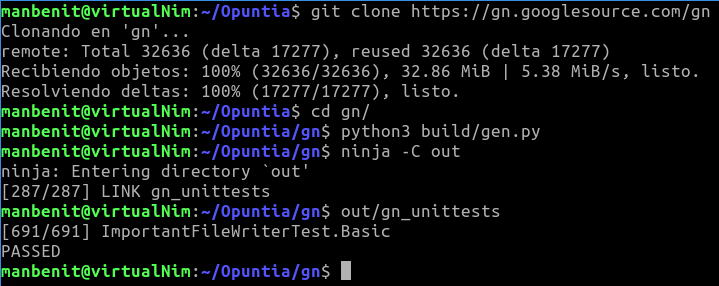
\includegraphics[scale=0.4]{installGn.png}
	\end{center}
\end{frame}

\begin{frame}{Instalación de LLVM}
	\begin{center}
		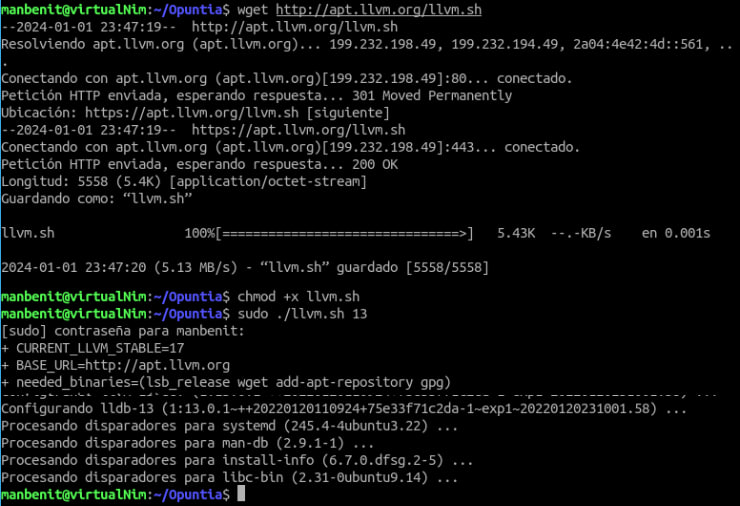
\includegraphics[scale=0.5]{installLlvm.jpg}
	\end{center}
\end{frame}

\begin{frame}{Instalación del \textit{toolchain} para x86}
	\begin{center}
		\ttfamily
		chmod 775 toolchains/scripts/i686-elf-tools.sh
		
		\enter
		
		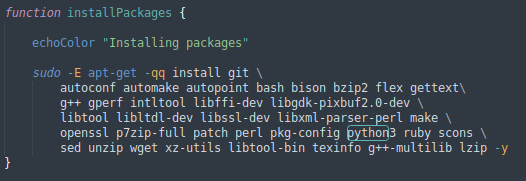
\includegraphics[scale=0.55]{modificarPython.png}
		
		\enter
		
		./toolchains/scripts/i686-elf-tools.sh
	\end{center}
\end{frame}

\begin{frame}{Instalación del \textit{toolchain} para x86}
	\begin{center}
		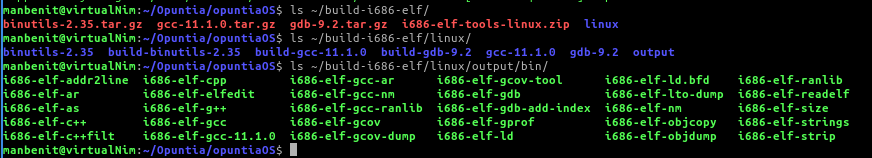
\includegraphics[scale=0.35]{toolchainx86_res.png}
		
		\enter
		
		\ttfamily
		export PATH=\$PATH:<directorio\_de\_contrucción>/linux/output/bin
	\end{center}
\end{frame}


\begin{frame}{Instalación de \textit{toolchain} para ARM}
	\begin{center}
		\ttfamily
		chmod 775 toolchains/scripts/arm-none-eabi-tools.sh
		
		\enter
		
		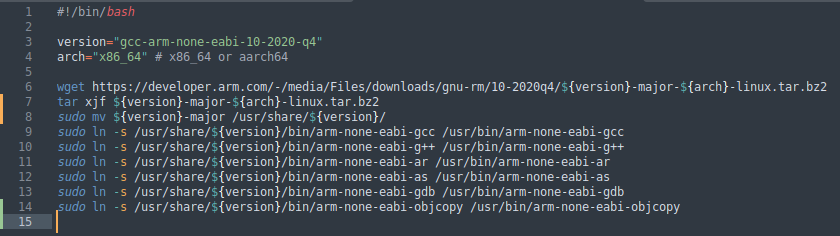
\includegraphics[scale=0.35]{modifArmSsh.png}
		
		\enter
		
		./toolchains/scripts/arm-none-eabi-tools.sh
	\end{center}
\end{frame}

\begin{frame}{Instalación del \textit{toolchain} para ARM}
	\begin{center}
		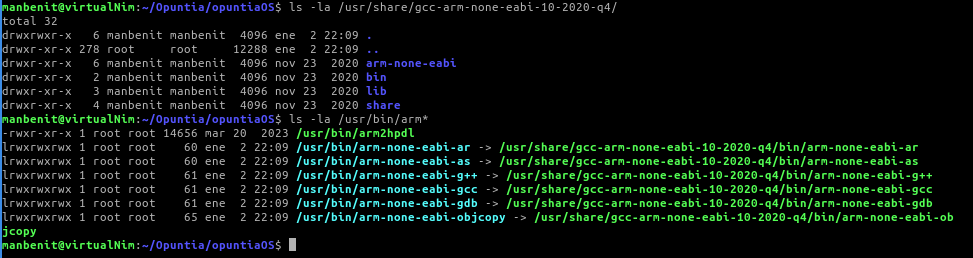
\includegraphics[scale=0.3]{toolchainArm_res.png}
	\end{center}
\end{frame}



%\section{Contrucción}

\section{Análisis}
\begin{frame}{}
	
\end{frame}

\begin{frame}{Implementación del \textit{bootloader}}
	Lo primero de lo que es posible percatarse al analizar la implementación del \textit{bootloader} es que la estructura de carpetas y archivos es distinta para \texttt{ARM} y \texttt{x86}.
	\begin{center}
		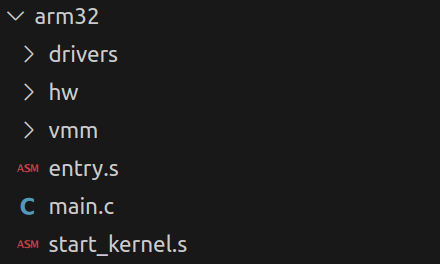
\includegraphics[scale=0.3]{estrucDir_ARM.png}
		\hspace{0.5cm}
		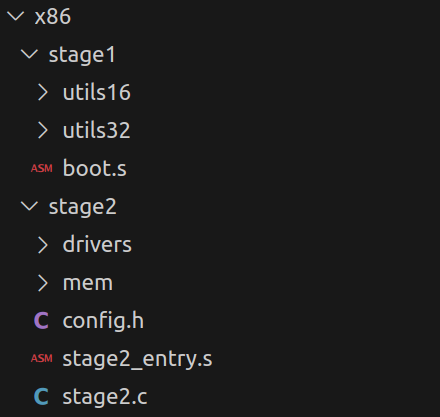
\includegraphics[scale=0.3]{estrucDir_x86.png}
	\end{center}
\end{frame}

\begin{frame}{Implementación del \textit{bootloader}}
	En el caso de \texttt{OpuntiaOS} para \texttt{x86}, se manejan 2 archivos de etapa para el arranque del sistema en lugar de 1, es decir, no se generará el archivo \texttt{stage2\_eltorito}, si no que se generarán 2 archivos de carga de \textit{kernel}.
	\begin{center}
		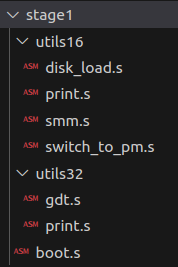
\includegraphics[scale=0.3]{x86_stage1_code.png}
		\hspace{0.5cm}
		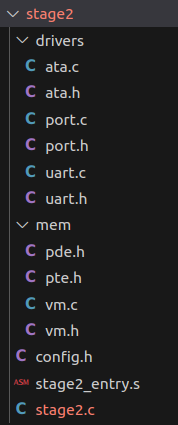
\includegraphics[scale=0.3]{x86_stage2_code.png}
	\end{center}
\end{frame}

\begin{frame}{}
	La primera etapa de carga contiene solo código ensamblador, es to es porque \texttt{stage1} se carga desde la BIOS y es la encargado de realizar la primera carga del \textit{kernel}, se puede decir que el archivo más importante es \texttt{boot.s}, similar a los \textit{kernel} compilados en el curso.
\end{frame}


\begin{frame}{Implementación del \textit{bootloader}}
	En el caso de \texttt{OpuntiaOS} para \texttt{ARM}, el \textit{bootloader} trabaja en 2 etapas, la primera en modo supervisor, que se encarga de acceder a los recursos del sistema y poder ejecutar el \textit{kernel} del sistema y la de modo usuario, donde se restringe el acceso a \textit{hardware}.
	\begin{center}
		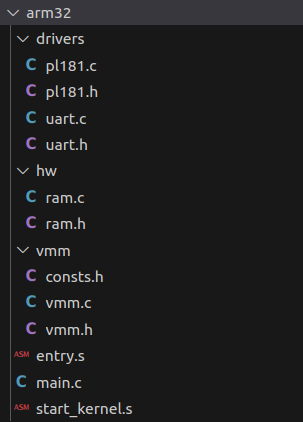
\includegraphics[scale=0.3]{arm_boot_code.png}
	\end{center}
\end{frame}

\begin{frame}{}
	La primera etapa de carga contiene solo código ensamblador, es to es porque \texttt{stage1} se carga desde la BIOS y es la encargado de realizar la primera carga del \textit{kernel}, se puede decir que el archivo más importante es \texttt{boot.s}, similar a los \textit{kernel} compilados en el curso.
\end{frame}




